\section{Design}
\label{sec:design}

This section presents the design of {\name}, including the overall architecture,
the data model, and the protocols for the {\em put}, {\em get} and {\em delete} operations.

\subsection{Overview and Challenges}

\begin{figure}[tp]
\centering
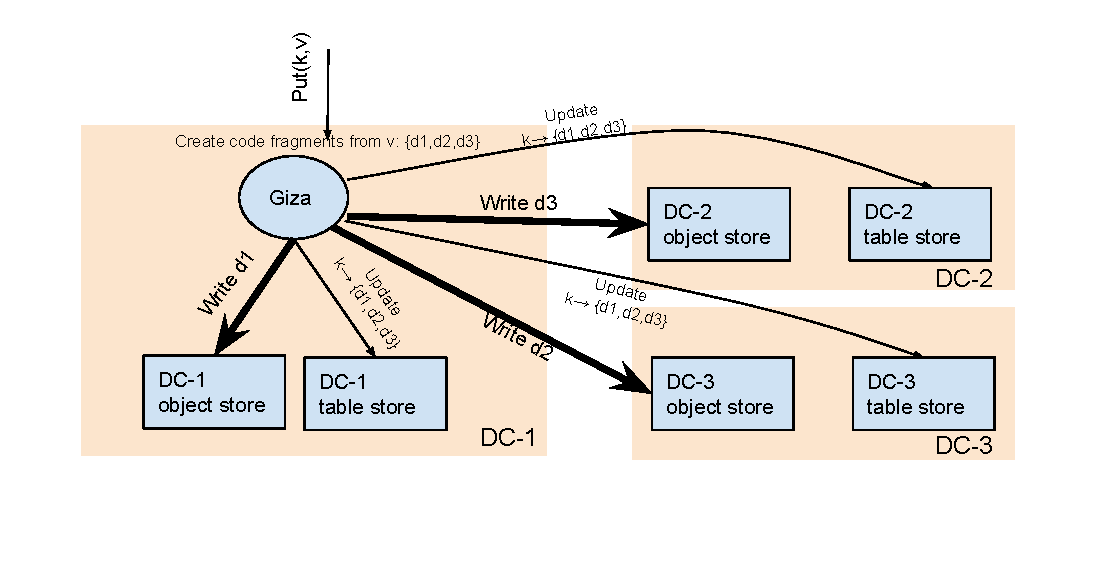
\includegraphics[width=0.52\textwidth]{fig/Giza}
\caption{Giza architecture\label{fig:arch}}
\end{figure}

\paragraph{Architecture}
{\name} is a global-scale cloud storage system that spans across many data
centers. It stores mutable, versioned objects. Figure~\ref{fig:arch} shows the
architecture of \name. To store a \name object through a {\em put} operation,
there is a data operation, and a metadata operation, both are carried out
simultanenously to improve the performance. On the data path, \name splits and
encodes the object into data and parity fragments. Each fragment is uniquely
named by its content hash and stored in a different DC. The design also ensures
that if there are multiple objects in a \name account, only one copy of the
object needs to be stored, thus achieves deduplication saving within the DC. It
is possible that the exact same fragments may be stored at different DC. \name
doesn't attempt to detect duplicate fragments across DC for performance concern.
Each Update to the object creates a new versions of the object. The version
numbers and the hashes of the coded fragments in each version constitutes the
metadata of the object. On the metadata path, \name replicates the metadata
across the data centers.

We implement \name on top of an existing cloud storage infrastructure. This
provides two advantages. First, doing so allows the rapid development of \name
by re-using mature, deployed and well-tested systems. Second, it simplifies the
failure recovery and the deployment of \name: the \name nodes are completely
stateless and can be readily integrated with the rest of the stateless cloud
storage front-ends.

%Existing cloud storage systems have redundancy within a single data center, but are not geo-replicated.  Thus, \name must explicitly provide cross data center redundancy through coding and replication.
% To write the object,
% {\name} stores the coded fragments in different data centers in cloud blob stores,
% such as Azure Blob, or AWS S3.
% Additionally, \name replicates the object's metadata across multiple data centers 
% and stores the metadata in cloud tables, such as Azure Table, or AWS DynamoDB. 
\name store data and coded fragments in cloud blob store, e.g., Azure Blob, and store the metadata in cloud table, 
e.g., Azure Table. 
The total number of the data plus coded fragments is equal to the number of data centers
storing the data objects, and is configured during the account setup depending on the user desired tradeoff on
durability vs. cost.
%The number of data centers to replicate the metadata is fixed at 3.

%blob service as building blocks, to store metadata and data respectively. This evolutional
%design allows {\name} to minimize footprint of new code. In fact, {\name} merely needs to replace the previous front-end
%module. With {\name} deployed, the user request comes in to the new frontend, where the new
%{\name} service will translate the user requests into a few metadata operations and data operations.
%
%In {\name}, both metadata and data are synchronously duplicated across different
%datacenters in order to tolerate datacenter failures. What is different between metadata
%and data is, metadata is fully replicated across a (usually smaller) set of datacenters using
%a tailored Fast-Paxos algorithm, persistent in the table service in each datacenter, thus
%tolerating a minority of failures; On the other hand, data in user request is encoded to
%a configurable number of fragments and shipped to a (usually larger) set of datacenters,
%persistent in the blob storage service. We refer the former as metadata path and the latter
%as data path.


\paragraph{Technical challenges}
% JinL: should we need to discuss ref counting & garbage collection when a fragment is no longer referenced? 
% Or is that considered well understood in the industry that we don't need to dicuss? 
In \name, each fragment (data or coded) is uniquely indexed by its content hashes.
As a result, each fragment is immutable, which makes the data path straightforward and simplified. 

The metadata path is more tricky, with the following three main technical challenges:
\begin{enumerate}

\item {\it Building a strongly consistent, geo-replicated metadata storage out of existing 
single-DC cloud tables.}
There are prototype systems, such as Cassandra,
that offer strongly consistent, geo-replicated storage systems.
Giza chooses not to adopt the existing solutions because
1) it is desirable to make \name nodes stateless and keep all data and metadata
in existing well-tested cloud storage infrastructure;
2) it is preferable to implement protocols best suited for our targeted workloads,
so as to achieve optimal latency.
Indeed, Giza ensures strong consistency by implementing the Paxos consensus protocol.
The trick is to implement Paxos using existing cloud table APIs and achieve 
optimal latency in the cross-DC setting.

\item {\it Jointly optimizing the data and metadata paths to achieve a single
  cross-DC round trip for read/write operations.} A naive approach would execute
  the data and metadata path sequentially: first write out the blob, completes
  the data path, and then starts on the metadata path. Doing so guarantees that
  the metadata written and externally visible always matches with the stored
  data. However, each write operation will require at least two cross-DC round
  trips. Similarly, a naive approach for read operation would take the first
  cross-DC round trip to retrieve the metadata and then the second round trip to
  retrieve the data. We want to combine the data and metadata path of \name to
  achieve a single cross-DC round trip for both read and write.

\item {\it Performing garbage collection efficiently and promptly.} When a data
  object is deleted, or its old versions are garbage collected, \name must
  remove obsolete fragments and/or metadata from the underlying cloud blob
  storage and cloud table. \name must also remove fragments generated by a
  failed data path write. Both operations are non-trivial because \name's
  garbage collection mechanism must be able to handle data center failures while
  ensuring data consistency and durability.

\end{enumerate}

%The separation of metadata path and datapath bring in the challenge that the consistency level
%could be violated with brutal yet flawed merge of the two. Our protocols described in later
%sections will guarantee the metadata path and data path together (especially when they are
%fully concurrent) will still provide a strong consistency insurance.
%


% A typical giza architecture for a data center includes the giza nodes, the Azure Blob Storage, and the Azure Table Storage. The giza nodes are the processing units of the Giza architecture and manages the data and the metadata. Furthermore the giza nodes participate in paxos rounds as coordinators. Figure 1 illustrates the architecture of Giza. Giza separates data from metadata and handles them on different paths. The data path is responsible for encoding the data and sending the data fragments across data centers. Each data fragment is stored in the corresponding DC’s Azure Blob Storage. The metadata path is responsible for storing the latest version of the data and the location of its data fragments. Giza uses a variant of the Paxos state machine replication (SMR) to maintain consistency of the metadata where each metadata server maintains a local copy of the replicated log. The replicated log is stored in the Azure Table Storage.

\subsection{Paxos using Cloud APIs}

The metadata operation of \name implements Paxos on top of an existing cloud
tables (Azure Table).

\subsubsection{Paxos and Fast Paxos: A Brief Primer and Implementation}

The Paxos algorithm~\cite{lamport01paxos} provides a mechanism to reach
consensus among a set of {\em acceptors} and one or more {\em proposers}. Each
proposer initiates a Paxos voting process by first picking a distinguished {\em
  ballot}. All ballots are unique and can be compared to each other. The
proposer sends requests to the acceptors, and associates each request with a
proposed value. Each acceptor decides whether to accept a request based on its
own state. The proposed value is {\em committed} when it is accepted by a {\em
  quorum} of the acceptors. The acceptors update their states when a request or
value is accepted. Paxos is typical implemented via active acceptors, which are
capable of comparing the ballot of an incoming request with its own state and
deciding whether to accept the request. In \name, we use the cloud tables as the
acceptors and implement the acceptor's logic as {\em atomic conditional updates
} to the table. This requires some modification of the proposer logic, which is
implemented at each \name node.

Paxos takes two {\em phases} to reach consensus, where {\em phase} $1$ prepares
a ballot and {\em phase} $2$ accepts a value. Since each phase takes one round
trip, applying Paxos in Giza results in two cross-DC round trips for metadata
writes~\footnote{Typical Paxos optimization elects a distinguished leader. The
  leader executes {\em phase} $1$ in advance and only takes one round trip in
  {\em phase} $2$ to reach consensus. This, however, requires relaying all
  updates through the leader. In the cross-DC scenario, it takes one cross-DC
  round trip to relay updates originating from non-leader DCs. Therefore, these
  updates still take two cross-DC round trips to commit.}.

Fast Paxos~\cite{lamport05fast} is a variation of Paxos that optimizes the
performance over cross-DC acceptors. It employs two types of rounds: fast round
and classic round. A fast round sends a PreAccept request and takes a single
round trip to reach consensus. A classic round resembles the two phases in Paxos
and takes two round trips. The fast round in Fast Paxos demands a larger quorum
than that in Paxos. Consider a case with $3$ acceptors. Paxos is able to reach
consensus with 2 out of the 3 acceptors (quorum size of 2). In comparison, Fast
Paxos only reaches consensus with all 3 acceptors (quorum size of 3). The
advantage is that if all 3 acceptors are working, the consensus can be reached
in a single round trip. The larger quorum requirement is acceptable in \name, as
its data path need to store fragments in a larger number of data centers to make
progress as well.

%Because Giza's data path requires multiple data centers to be online to make progress, 
%In Giza, the success of the data path requires multiple data centers to be online to make progress, it turns out easy to satisfy the demand of a larger quorum, and suites the implementation need in Fast Paxos. E.g., Giza requires at least 3 data centers to stripe the coded fragments (with $2 + 1$ erasure coding). Hence, the data path won't succeed unless there are at least 3 data centers available, which makes it easy to satisfy the larger quorum requirement.

Giza implements both Paxos and Fast Paxos. We discusses the Fast Paxos only, as
it is more tricky (but more performant) than Paxos.
%Hence, the most optimized metadata path in Giza implements Fast Paxos, as detailed next.

\begin{figure}[tp]
\centering
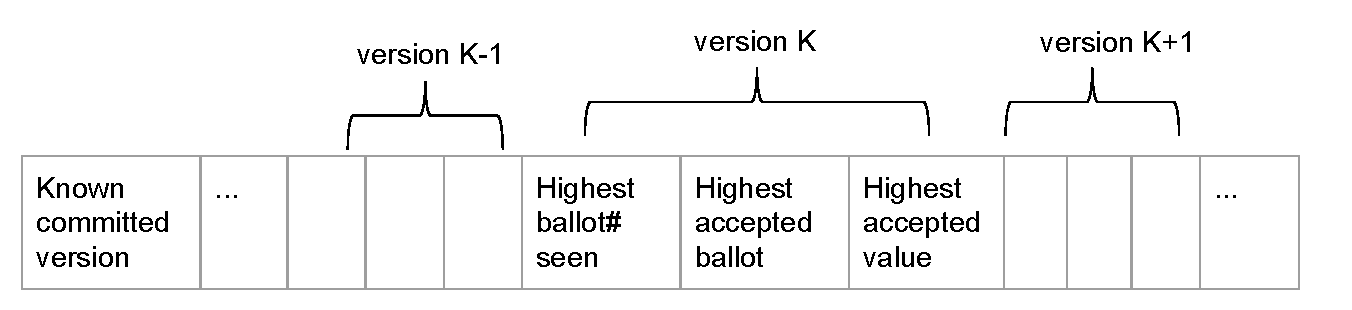
\includegraphics[width=0.5\textwidth]{fig/Giza_Metadata}
\caption{For each object, \name stores the Paxos protocol state and the object metadata 
in a single row in the underlying cloud table.\label{fig:metadataschema}}
\end{figure}

\subsubsection{Metadata Storage Layout}

%\name implements the Paxos consensus protocol to serialize the operations on each data object.
% To implement the Paxos consensus protocol,
\name needs to persist the Paxos states together with the metadata for the object in the cloud table. 
We use one table row per object, with a dynamic number of columns, with each three columns corresponding to one version of the object. The layout of each table row is
shown in Figure~\ref{fig:metadataschema}.

Each object version is represented by a consecutive natural numbers, starting
from $1$. Every \name write to the same object creates a new version. For each
version, \name launches a separate Paxos proposal, and uses Paxos to guard
against races among other \name writers and cloud table failures. For a data
object, the metadata of all versions and the states of all the Paxos instances
are stored in the same table row. Specifically, the metadata contains a triplet
of columns for each version of the object (Figure~\ref{fig:metadataschema}). Two
of them are Paxos states: {\tt highest ballot seen} and {\tt highest accepted
  ballot}. The other column, {\tt highest accepted value}, stores the metadata,
including the erasure coding scheme, the hash of each fragment (data or parity),
and which DC the fragment is stored at.

{\name} additionally maintains a set of {\tt known committed versions} for all
those that have been committed by Paxos. This is to facilitate both {\em put}
and {\em get} operations and will be discuessed in the following sections.
%As will become clear later,
%this set provides a hint to facilitate both write and read operations.
%It is a hint in the sense that newly committed versions are added to the set asynchronously,
%or beyond the critical path of write operations.
%Hence, while all the version numbers in the set are guaranteed to have been committed,
%the latest committed version number might yet have to be included.

\subsubsection{Metadata Write - Common Case}

The metadata path begins by choosing a proper new version number to run the Fast
Paxos~\cite{lamport05fast} algorithm. Since version numbers are consecutive, the
new version should succeed the most recently committed version. While it is safe
to use an outdated version (in which case the {\name} node will later realize
its mistake and retry with a higher version number), it is unsafe to choose a
higher one resulting in non-consecutive versions. The {\name} node identifies
the proper version in an optimistic fashion. Specifically, it reads {\tt known
  committed versions} from the table in its local DC, then uses the next higher
number as the chosen version number to launch a Fast Paxos round. A PreAccept
request is sent to all cloud tables, each located in a different DC. Each
request is an {\em atomic conditional update} on the table row of the object. If
there are no competing write requests to the same object, the PreAccept request
will succeed in updating the table row. Otherwise, the PreAccept request will be
rejected by the table and leave the table row unchanged. Section~\ref{sec:impl}
illustrates how atomic conditional update is implemented leveraging existing
cloud APIs.

Whenever the {\name} node receives a {\em fast quorum} of positive PreAccept
responses, the corresponding version is considered to have been committed. The
{\name} node asynchronously sends a Commit confirmation to all the cloud tables
to update the set of {\tt known committed versions} to include the recently
committed version. The Commit confirmation is again an atomic conditional
update, which only succeeds if the version number is not yet included in the
current set.

Since the Commit confirmation is completed asynchronously, the critical path
only involves the PreAccept request and response. Hence, without conflict, the
above described metadata write involves only one cross-DC round trip and is
referred to as the {\em fast path}.
% When there is no contention, the fast path always succeeds.

\subsubsection{Metadata Write with Contention}

The fast path may fail when the {\name} node fails to collect a fast quorum of
positive PreAccept responses. This may result from concurrent updates to the
same object (contention), or because one or more cloud tables fail. In this
case, {\name} enters what is referred to as a \emph{slow path} to perform
classic Paxos in order to guarantee safety in case of contention.

On the slow path, the {\name} node first picks a distinguished ballot number and
then replicates a Prepare request to write the ballot to all the metadata tables
and wait for a majority of responses. The Prepare request is a conditional
update operation. The operation succeeds only if the {\tt highest ballot seen}
is no more than the ballot in the Prepare request. The operation also returns
the entire row as a result.

Upon collecting a majority of successful replies, the {\name} node needs to pick
a value to commit. The rule for picking the value is categorized into three
cases. In case 1, Giza looks for the highest accepted ballot in the replies. If
there is one, the value from the reply is picked. In case 2, the replies contain
no accepted value, but rather pre-accepted values. Giza picks the pre-accepted
value that appears more than others (if any) from the replies. Both case 1 and 2
imply the possibility of an ongoing Paxos instance, so Giza picks the value so
as to complete the Paxos instance first. It then starts with a new version and
follows the fast path to commit its current metadata. In case 3, there is
neither pre-accepted nor accepted value, which implies no real impact from
contention. Giza picks its current metadata as the value and proceeds to next
steps.

% JinL: my understanding is that Azure Table's conditional update is based on etag. 
% That is, the conditional update is performed if old_etag = cur_etag, and is rejected otehrwise. 
% It can't perform a function to check whether {\tt highest ballot seen} and/or {\tt highest accepted ballot} 
% is alrger. 
Once the {\name} node picks a value, it replicates an Accept request to all the
metadata tables. The accept request is again an atomic conditional update; it
succeeds in writing {\tt highest accepted ballot} and {\tt highest accepted
  value} if neither {\tt highest ballot seen} and {\tt highest accepted ballot}
is larger. 
As soon as a majority of Accept requests succeed, the \name node
considers the corresponding metadata write completed and sends acknowledgment to
clients. Additionally, a Commit confirmation is replicated in the background, as
described before.

\subsubsection{Metadata Read}

To get the metadata of the \emph{latest} object version, it is insufficient for
\name to only read the corresponding metadata table row from its local DC. This
is because the local DC might not be part of the majority quorum that has
accepted the latest version. To ensure correctness, Giza needs to read the
metadata rows from more than one DC.

In the common case, {\tt known committed versions} is already updated and
includes the latest committed version (say version $k$). The metadata table row
from the local DC obtains version $k$. And the metadata table row from a
non-local DC confirms the lack of higher committed versions than $k$. Hence, in
the case that the metadata is replicated to 3 DCs, the metadata from 2 DCs (one
local and one non-local) leads to a decisive conclusion that version $k$ is the
latest committed version. It is therefore safe for the Giza node to return
version $k$ to clients.

In general, the \name node reads the metadata table rows from all the DCs.
Whenever a majority rows have matching {\tt known committed versions} and have
not accepted any value for a higher version, the \name node returns the metadata
of the highest committed version.

If the replies contain an accepted value with a higher version number than the
{\tt known committed versions}, the \name node needs to follow a slow path
similar to the one in the write operation. This is to confirm whether the higher
version has been committed.
%despite that the version is not included in {\tt known committed versions} and the metadata tables in certain DCs may have missed the quorum.

%This is because it could possibly be considered committed once before. After it succeed in the slow path, the {\name} node needs to re-launch the datapath to retrive the data fragments of the newer version and abandon the old ones. This serialized metadata and datapath case typically happens when there is concurrent read and write on the same object, which is rare in our workload.

%\sm{ Hi Daniel, just want to confirm, is this what you do now? Only one accepted in higher version will invalidate the optimistic read}

% continue to design_part2.tex
